\documentclass[11pt]{extarticle}
\usepackage{mathtools}
\usepackage[a4paper, total={6in, 8.5in}]{geometry}
\usepackage{graphicx}
\usepackage{subfig}
\usepackage{amssymb}
\usepackage{amsmath}
\usepackage{pythonhighlight}
\usepackage{pdfpages}
\usepackage[T1]{fontenc}
\usepackage[utf8]{inputenc}
\usepackage{fancyhdr}
\usepackage{pythonhighlight}
\usepackage{changepage}
\usepackage{slashbox}
\usepackage{floatrow}
\floatsetup[table]{capposition=top}

\sloppy
\definecolor{lightgray}{gray}{0.5}
\setlength{\parindent}{0pt}
\setlength{\headheight}{14pt}

\renewcommand{\headrulewidth}{.4mm} % header line width
\newcommand{\norm}[1]{\left\lVert#1\right\rVert}


\pagestyle{fancy}
\fancyhf{}
\fancyhfoffset[L]{-1cm} % left extra length
\fancyhfoffset[R]{-1cm} % right extra length
\rhead{\bfseries Kutay U\u{g}urlu 2232841}
\lhead{EE583 Homework 1}
\rfoot{}

\DeclarePairedDelimiter\ceil{\lceil}{\rceil}
\DeclarePairedDelimiter\floor{\lfloor}{\rfloor}

\author{Kutay U\u{g}urlu 2232841}
\begin{document}   


\fancyfoot[C]{\thepage}
\title{\LARGE \LARGE EE583 Pattern Recognition HW1}

\maketitle{\LARGE}

\pagebreak
\section*{Question 1}

{\centering
    \begin{figure}[h]
        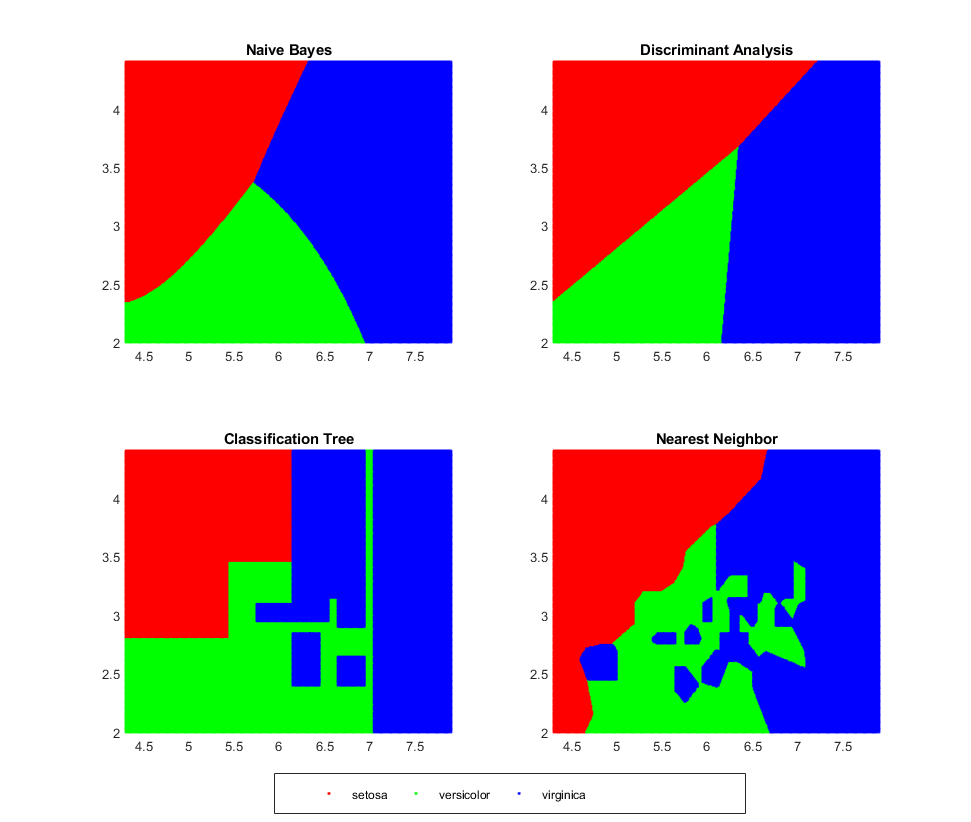
\includegraphics[width=12cm, height=8cm]{q1_output.png}
        \caption{Decision boundaries for flower classes}
        \label{fig:q1figure}
    \end{figure}
}

In Figure \ref{fig:q1figure}, boundaries of 4 different classifiers are shown. Boundaries of Nearest Neighbors and Classification tree
seem to overfit the data, \textit{i.e.}, it memorized the training data and boundaries have high variability to fit it. On the other
hand, the boundaries of the remaining classifiers show that they are better at generalizing, \textit{i.e.}, they make better statistical 
inferences on the data that model has never seen, test data. In addition, Discriminant Analysis classifier has almost linear decision 
boundaries, in contrast to Na\"ive Bayes. \\
I would choose Na\"ive Bayes classifier in such a classification task. Although it has comparable performance with Na\"ive Bayes for class 
\textbf{setosa}, the decision boundary between the remaining two classes is represented better by the Na\"ive Bayes classifier in terms of 
generalization. 

\pagebreak

\section*{Question 2}

\begin{center}
    \begin{figure}[h]
        \begin{tabular}{cc}
        \subfloat[Prior Probabilities = 0.33,0.33,0.33]{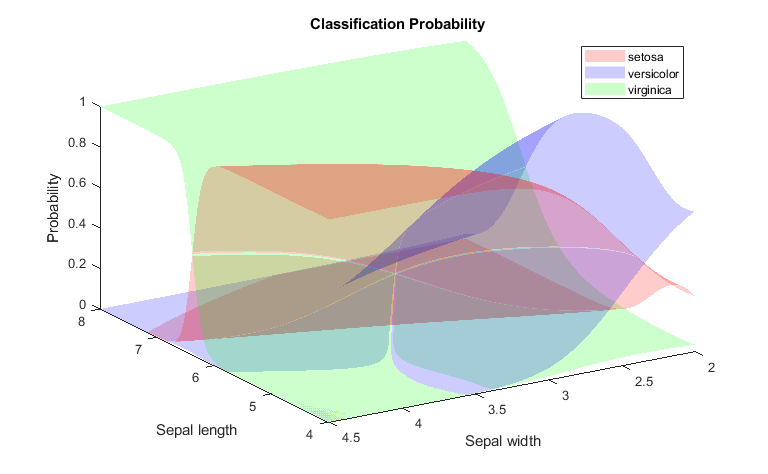
\includegraphics[width = 2.5in]{eq.png}} &
        \subfloat[Prior Probabilities = 0.10,0.15,0.75]{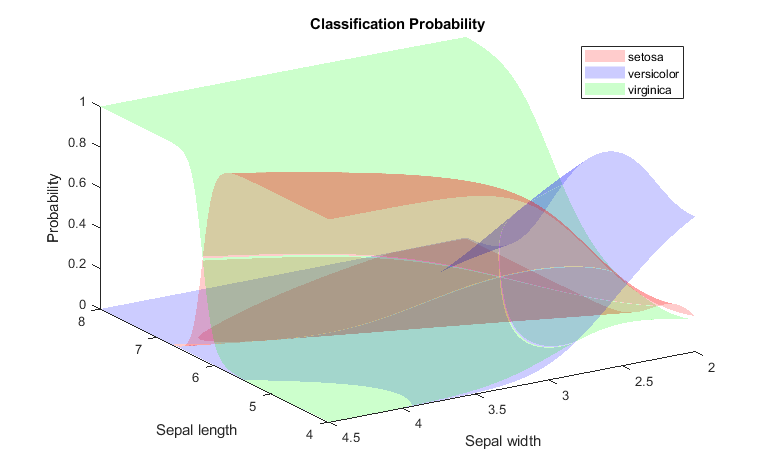
\includegraphics[width = 2.5in]{01015075.png}} \\
        \subfloat[Prior Probabilities = 0.10,0.75,0.15]{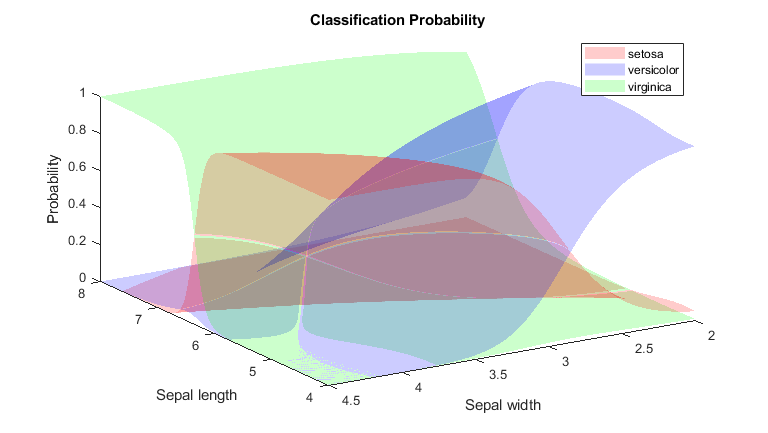
\includegraphics[width = 2.5in]{01075015.png}} &
        \subfloat[Prior Probabilities = 0.75,0.10,0.15]{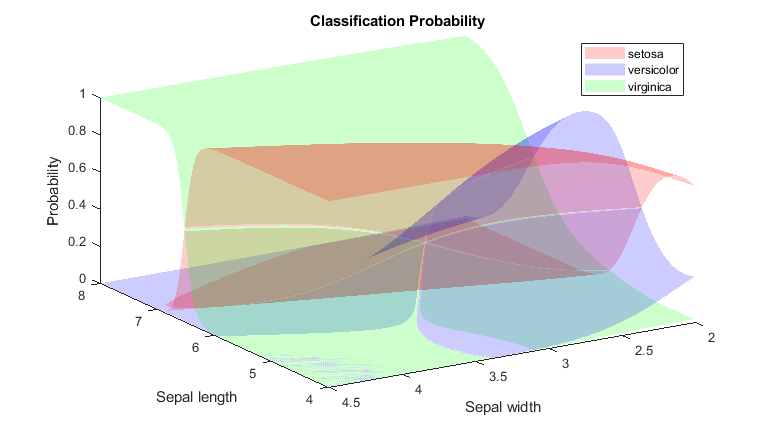
\includegraphics[width = 2.5in]{07501015.png}} \\
        \end{tabular}
        \caption{Posterior probabilities based on different priors}
        \label{q2fig}
    \end{figure}
\end{center}

\begin{equation}
    p(w_j|x) = \frac{p(x|w_j)P(w_j)}{p(x)}
    \label{posterior_eqn}
\end{equation}

Considering the posterior distribution given in Eqn. \ref{posterior_eqn}, the value gets bigger for a fixed class and feature vector
when prior probability of a class, $p(w_j)$ is increased. Hence, it is investigated that the portion of the feature space where class
setosa gets the probability of 1 largely increased when figures a and d are compared. Same observation can also be made for 
versicolor class in the comparison of figures b and c.

\pagebreak 

\section*{Question 3}

{\centering
    \begin{figure}[h]
        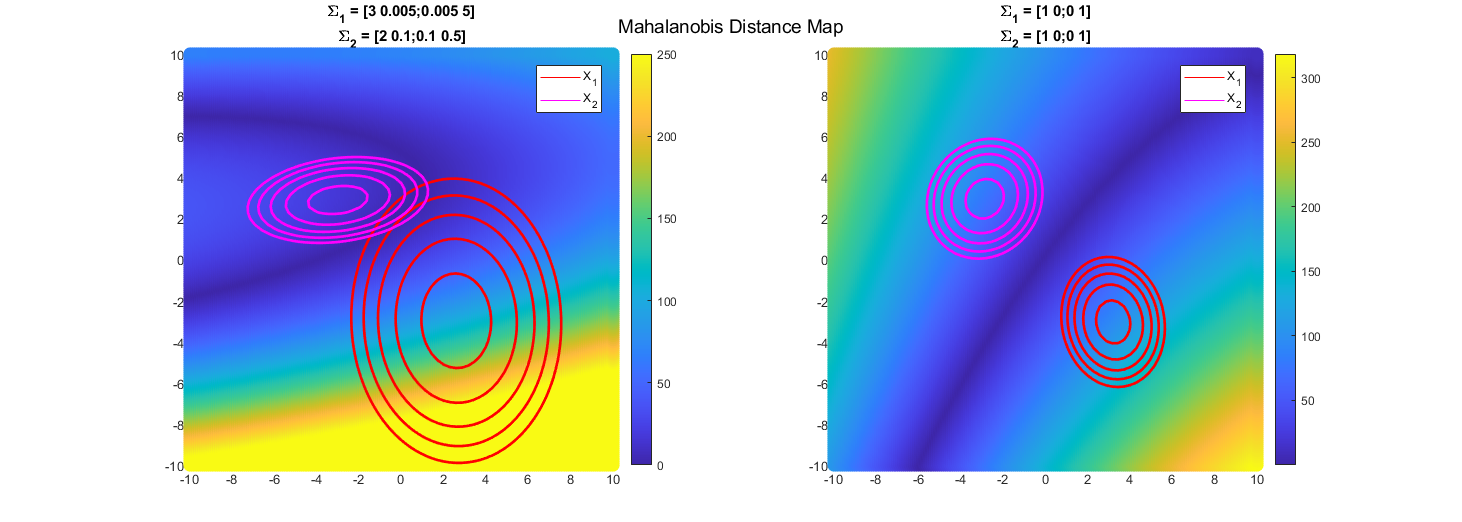
\includegraphics[width=16cm, height=6cm]{mahal.png}
        \caption{Mahalanobis Distances for 2 normal distributions}
        \label{fig:q3figure}
    \end{figure}
}

For the given covariance matrices in Figure \ref{fig:q3figure}, Mahalanobis distances are plotted to the
background of the figure. The boundary where Mahalanobis distance is around 0 is observed to have a 
quadratic shape, whereas it is almost linear in the plot on the right. 

\section*{Question 4}

\begin{center}
    \begin{figure}[h]
        \begin{tabular}{ccc}
        \hspace*{-2.3cm}\subfloat[ROC1]{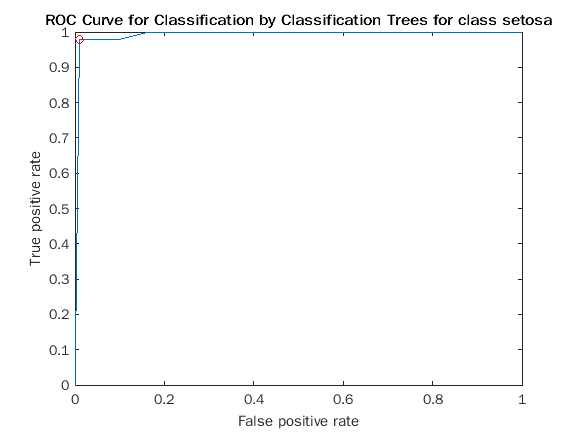
\includegraphics[width = 2.5in]{1.png}} &
        \subfloat[ROC2]{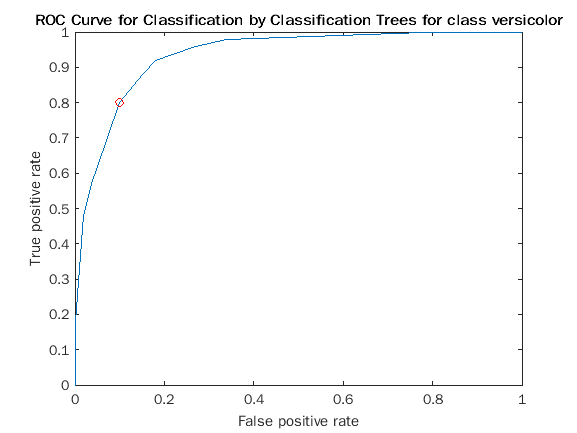
\includegraphics[width = 2.5in]{2.png}} &
        \subfloat[ROC3]{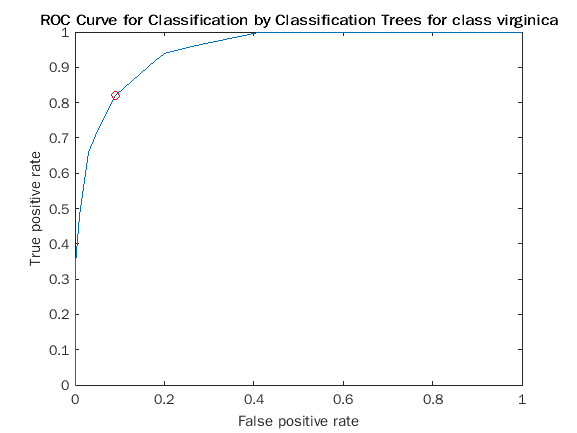
\includegraphics[width = 2.5in]{3.png}} \\
        \end{tabular}
        \caption{ROC curves for different class predictions}
        \label{q4fig}
    \end{figure}
\end{center}

\end{document}

